% !TeX root = main.tex
\documentclass[12pt]{article}
\title{Investigating positional accuracy by double integrating accelerometer data}
% \author{Jimmy Zeng}

\usepackage{listings}
\usepackage{xcolor}
\usepackage{minted}
\usepackage{amsmath}
\usepackage{pgfplots}
\usepackage{tikz}
\usepackage{graphicx}
\graphicspath{{images/}}
\usetikzlibrary{patterns}
\pgfplotsset{compat=1.18, width=10cm}

\newcommand{\diff}{\ensuremath{\operatorname{d}\!}}

\definecolor{icegreen}{HTML}{20D68A}
\definecolor{iceteal}{HTML}{16C7B7}
\definecolor{icecyan}{HTML}{18C9E8}
\definecolor{iceblue}{HTML}{239FE8}
\definecolor{icedark}{HTML}{202B32}
\definecolor{icegray}{HTML}{C9D0D3}


\begin{document}
\maketitle
\pagebreak
\tableofcontents
    \section{Introduction}
        Inertial Odometry has been studied with a variety of applications, whenever you need to know the precise location of something instantly, chances are that double integrating accelerometer data outpaces GPS solutions. From robotics to step trackers, they all rely on the property that the area under a accelerometer graph can provide enough data used to compute the displacement of the object. In this investigation we will explore the accuracy of double integrating accelerometer data recorded on a phone during travel to find path traveled to get to school and create a visual representation of the position with respect to time and comparing with GPS data.

        \pagebreak
    \section{Numerical Integration and code application}
        Recall that in kinematics integrating acceleration gives velocity, and integrating once again gives displacement. For discrete-time data, this cannot be solve analytically. Instead we refer to the trapezoidal method, illustrated below:
\begin{figure}[h]
    \center
    
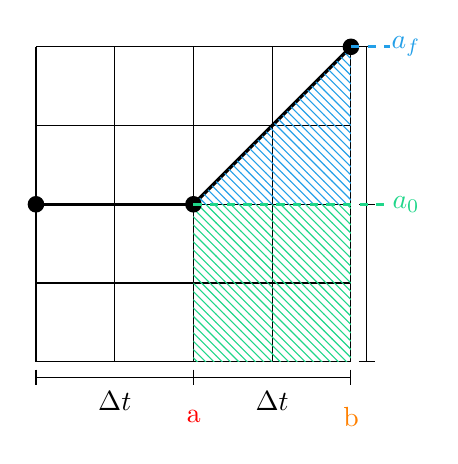
\begin{tikzpicture}
    \draw[step=1cm] (0,0) grid (4,4);
    \draw [black, very thick] (0,2) -- (2, 2);
    \draw [black, very thick] (2,2) -- (4,4);
    % \fill[pattern=north east lines, pattern color=green] (0,0) rectangle (2,2);
    \fill[pattern=north west lines, pattern color=icegreen] (2,0) rectangle (4,2);
    \fill[pattern=north west lines, pattern color=iceblue] (2,2) -- (4,2) -- (4,4) -- cycle;
    \fill (0,2) circle (3pt);
    \fill (2,2) circle (3pt);
    \fill (4,4) circle (3pt);
    \draw [black] (0, -0.1) -- (0, -0.3);
    \draw [black] (0, -0.2) -- (2, -0.2);
    \draw [black] (2, -0.1) -- (2, -0.3);
    \draw [black] (2, -0.2) -- (4, -0.2);
    \draw [black] (4, -0.1) -- (4, -0.3);
    \node at (1, -0.5) {$\Delta t$};
    \node at (3, -0.5) {$\Delta t$};
    \draw [black] (4.1, 0) -- (4.3, 0);
    \draw [black] (4.2, 0) -- (4.2, 2);
    \draw [black] (4.1, 2) -- (4.3, 2);
    \draw [black] (4.2, 2) -- (4.2, 4);
    \draw [black] (4.1, 4) -- (4.3, 4);
    \node [icegreen] at (4.7, 2) {$a_{0}$};
    \node [iceblue] at (4.7, 4) {$a_{f}$};
    \draw [icegreen, dashed, very thick] (2, 2) -- (4.5, 2);
    \draw [iceblue, dashed, very thick] (4, 4) -- (4.5, 4);
    \node [red]at (2, -0.7) {a};
    \node [orange]at (4, -0.7) {b};
\end{tikzpicture}
    \caption{Integrating two data points}
    \label{fig:trapezoidal integration}
\end{figure}

To calculate the area bounded by the x axis and the line created from two datapoints, we use basic geometry equations

\begin{equation}
    \Delta v = \int_{a}^{b} a(t)\diff t = \Delta t \cdot a_{0} + \frac{1}{2} \Delta t \cdot a_{f}
\end{equation}

which is thus computed in python code

% \begin{minted}{python}
% dt = final_time - initial_time
% dx_accel = final_accel - initial_accel
% dx_vel = (dt * initial_accel) + ((1/2) * dt * dx_accel)
% # triangle area + square area = area under accel graph = change in velocity
% \end{minted}


\subsection{Testing the waters}
    

the same idea will be repeated for each axis and afterwards applied to the calculated velocity values to find displacement. For this first model I moved my phone left and right 5 times on my table starting and ending at 0 velocity.

\begin{figure}[htbp]
    \center
    
    \begin{tikzpicture}
        \begin{axis} [
            % xmin = 0,
            % xmax = 10,
            % ymin = -10,
            % ymax=10,
            width = \textwidth,
            height = 5cm,
            axis lines = middle,
            xticklabel style = {yshift = -15},
            title = {Raw Accelerometer-Time Graph ("X" Direction)}
        ]

            \addplot[color=icegreen,very thick]
            table[
                x=Time,
                y=x,
                col sep=comma
            ]{data/best.csv};
        \end{axis}
    \end{tikzpicture}
    \caption{Raw accelerometer data on the X axis}
    \label{fig:raw-x-acceleration}
\end{figure}

And integrating the x-axis with the aforementioned algorithm we get this series of integrations
 expressed graphically (Assume this part will be corrected to the values given by the actual)

\begin{figure}[htbp]
    \center
    \begin{tikzpicture}
        \begin{axis} [
            % xmin = 0,
            % xmax = 10,
            % ymin = -10,
            % ymax=10,
            width = \textwidth,
            height = 5cm,
            axis lines = middle,
            xticklabel style = {yshift = -15},
            title = {Raw Accelerometer-Time Graph ("X" Direction)}
        ]

            \addplot[color=icegreen,very thick]
            table[
                x=Time,
                y=x,
                col sep=comma
            ]{data/test1/accel.csv};
        \end{axis}
    \end{tikzpicture}
    
    \begin{tikzpicture}
        \begin{axis} [
            % xmin = 0,
            % xmax = 10,
            % ymin = -10,
            % ymax=10,
            width = \textwidth,
            height = 5cm,
            axis lines = middle,
            title = {Integrated Velocity-Time Graph}
        ]

            \addplot[color=icecyan,very thick]
            table[
                x=Time,
                y=x,
                col sep=comma
            ]{data/test1/vel.csv};
        \end{axis}
    \end{tikzpicture}

    \begin{tikzpicture}
        \begin{axis} [
            % xmin = 0,
            % xmax = 10,
            % ymin = -10,
            % ymax=10,
            width = \textwidth,
            height = 5cm,
            axis lines = middle,
            title = {Integrated Displacement-Time Graph}
        ]

            \addplot[color=iceblue,very thick]
            table[
                x=Time,
                y=x,
                col sep=comma
            ]{data/test1/displ.csv};
        \end{axis}
    \end{tikzpicture}
    \caption{The Progressive Progress of Numerically integrating accelerometer data}
    \label{fig:int1}
\end{figure}
\pagebreak

Plugging into desmos for Sinusoidal regression we get:
\begin{equation}
    y=0.14272\cdot\sin\left(6.6486x+0.216978\right)-0.00389886
\end{equation}

\begin{figure}[htbp]
    \centering
    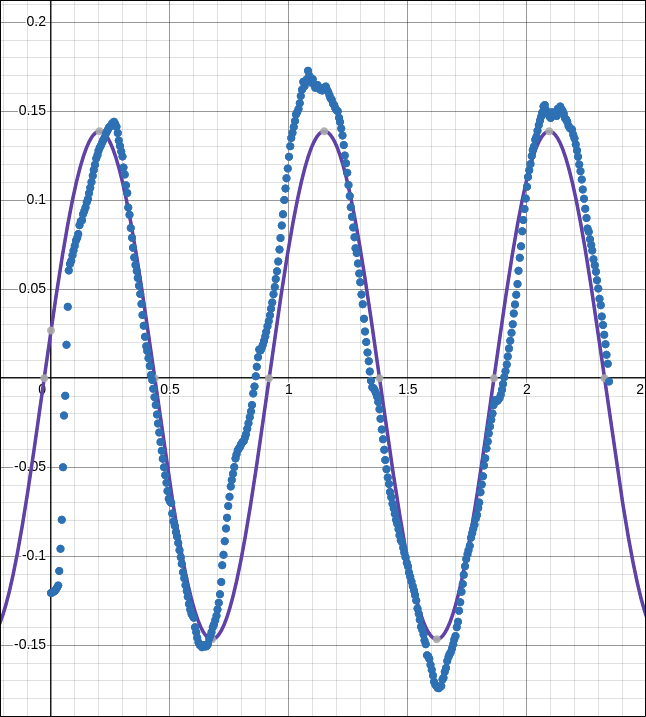
\includegraphics[width=.75\textwidth]{desmos}
    \caption{graph of our accelerometer data and the fitted curve}
    \label{fig:desmos}
\end{figure}
seen in figure \ref{fig:desmos}.
We will integrate this analytically twice:
\begin{equation}
    v(t) = \int \left(a\cdot\sin\left(bt+c\right)-d\right)\diff t
\end{equation}
where a, b, c, and d are constants. Rearranged, we get
\begin{equation}
    v(t) = a \int \sin(bt+c)\diff t - \int d \diff t
\end{equation}
Using u-substitution
\begin{align}
    u &= bt+c \\
    \frac{\diff u}{\diff t} &= b \\
    \diff t &= \frac{\diff u}{b}
\end{align}
plugging in u and dt:
\begin{align}
    v(t) &= a \int \sin(bt+c)\diff t - \int d \diff t \\
    &= a \int \sin(u) \frac{1}{b} \diff u - \int d \diff t \\
    &= \frac{a}{b}\int \sin(u)  \diff u - \int d \diff t \\
    &= -\frac{a}{b}\cos(u) - \int d \diff t \\
    &= -\frac{a}{b}\cos(bt+c) - dt + C_{1}
\end{align}
and since we know the constant represents the initial velocity, and since we start at rest, we need to find the constant $C_{1}$ such that $v(0)=0$
\begin{align}
    v(0) &= -\frac{a}{b}\cos(\left(0\right)b+c) - \left(0\right)d + C_{1} = 0 \\
    \frac{a}{b}\cos(c) &= C_{1} = 0.0209628448456 \\
\end{align}
For now, we will keep in mind that $C_{1} = 0.0209628448456$ but continue using $C_{1}$ throughout integration for convenience. To find the displacement function with respect to time we integrate again.
\begin{align}
    s(t) &= \int \left(-\frac{a}{b}\cos(bt+c) - dt + C_{1}\right) \diff t \\
    s(t) &= -\frac{a}{b} \int\cos(bt+c)\diff t - \int dt\diff t + \int C_{1}\diff t \\
    s(t) &= -\frac{a}{b} \int\cos(bt+c)\diff t - \int dt\diff t + \int C_{1}\diff t \\
\end{align}
Using the same u-substitution:
\begin{align}
    s(t) &= -\frac{a}{b} \int\cos(u)\frac{\diff u}{b} - \int dt\diff t + \int C_{1}\diff t \\
    s(t) &= -\frac{a}{b^{2}} \sin(u) - \int dt\diff t + \int C_{1}\diff t + C_{2} \\
    s(t) &= -\frac{a}{b^{2}} \sin(bt+c) - \int dt\diff t + \int C_{1}\diff t + C_{2} \\
    s(t) &= -\frac{a}{b^{2}} \sin(bt+c) - \frac{dt^{2}}{2} + C_{1}t + C_{2} \\
\end{align}
and since this data is filmed as relative displacement from original point (seen as 0) we need to find the value of $C_{2}$ such that $s(0)=0$. [Ai said wording was bad, I don't understand why]
\begin{align}
    s(0) &= -\frac{a}{b^{2}} \sin(b\left(0\right)+c) - \frac{d\left(0\right)^{2}}{2} + C_{1}\left(0\right) + C_{2} = 0 \\
    0 &= -\frac{a}{b^{2}} \sin(b\left(0\right)+c) + C_{2} \\
    \frac{a}{b^{2}} \sin(b\left(0\right)+c) &= C_{2} = 0.000695067592524 \\
\end{align}
Again we will keep $C_{2}=0.000695067592524 $ in mind.
Resulting in a final function $s(t)$:
\begin{equation}
    s(t) = -\frac{a}{b^{2}} \sin(bt+c) - \frac{dt^{2}}{2} + C_{1}t + C_{2}
\end{equation}
drawing a graph of progressive integration is seen in figure \ref{fig:model representation}
\begin{figure}[H]
    \center
    \begin{tikzpicture}
        \begin{axis} [xmin=0, xmax=5, ymin=-0.2, ymax=0.2, samples=2000]
            \addplot[mark=none, color=icegreen] {-0.00322867571063*sin(6.6486*x+0.216978) + 0.00389886*x^2 + 0.0209628448456*x + 0.000695067592524};
        \end{axis}
    \end{tikzpicture}
    \caption{graph of the model being integrated twice}
    \label{fig:model representation}
\end{figure}
????

We have a displacement/time graph from video. However it is a different sampling rate (120hz) than the recorded datapoints (100hz). Hence we will attempt to align by drawing a line between the points in the recorded accelerometer data, and interpolate the value.

\begin{figure}[htbp]
    \center
    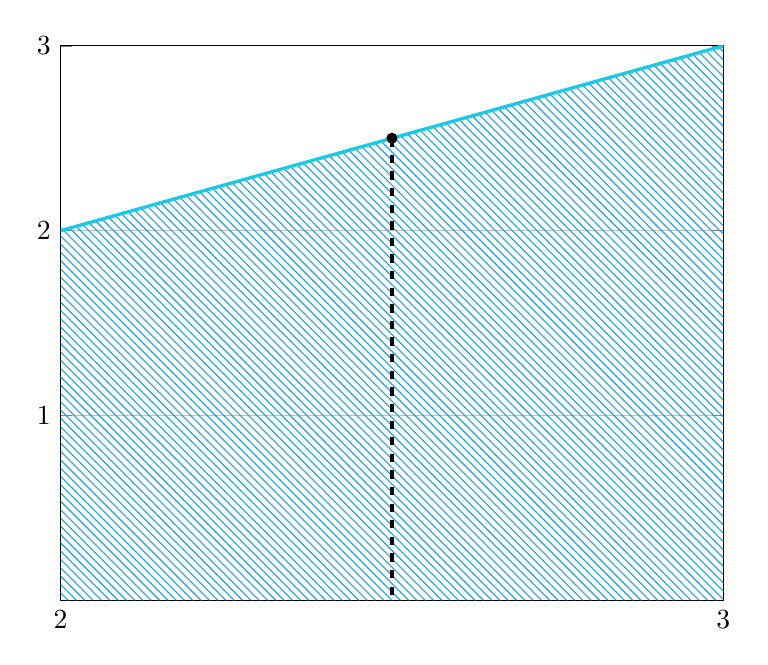
\begin{tikzpicture}
        \begin{axis} [xmin=2,xmax=3,ymin=0,ymax=3,grid=major,xtick={1,2,3},ytick={1,2,3}]
            \fill[pattern=north west lines, pattern color=iceblue] (2,2) -- (3,3) -- (3,0) -- (2,0) -- cycle;
            \draw [color=icecyan,very thick] (2,2) -- (3,3);
            \draw [color=black,very thick,dashed] (2.5,2.5) -- (2.5,0);
            \fill (2.5, 2.5) circle (2pt);
        \end{axis}
    \end{tikzpicture}
    \caption{Illustration of interpolating values from two datapoints $x=2,3$}
    \label{fig:interpolating values}
\end{figure}




\end{document}
